\documentclass{article}

\usepackage[sans, stdmargin, noindent]{../../rajeev}
\usepackage{listings}
\usepackage{graphicx}

\lstset{style=mystyle}

\pagestyle{fancy}
\rhead{\today}
\lhead{Math 291H HW \#1}

\begin{document}

\begin{center}
    \Large \textbf{Math 291H Computational Problem \#1}
\end{center}
  
\begin{center}
    \Large Rajeev Atla
\end{center}


\problem{1}

\lstinputlisting[language=Python, firstline=2, lastline=19]{lab1.py}

\problem{2}
\lstinputlisting[language=Python, firstline=23, lastline=44]{lab1.py}

From the dot product, we find $\theta \approx 2.802$.
From the cross product, we find $\theta \approx 0.340$.
Note that these angles add up to $\pi$.

\problem{3}
\lstinputlisting[language=Python, firstline=46, lastline=47]{lab1.py}

$\bm{v} = \pars{-1, 1, 0}$ is a vector that is orthogonal to both $\bm{pq}$ and $\bm{qr}$.

\problem{4}
\lstinputlisting[language=Python, firstline=49, lastline=72]{lab1.py}

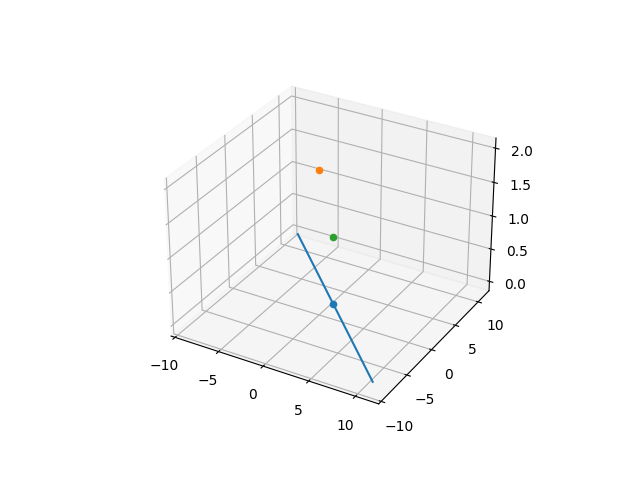
\includegraphics{fig1.png}

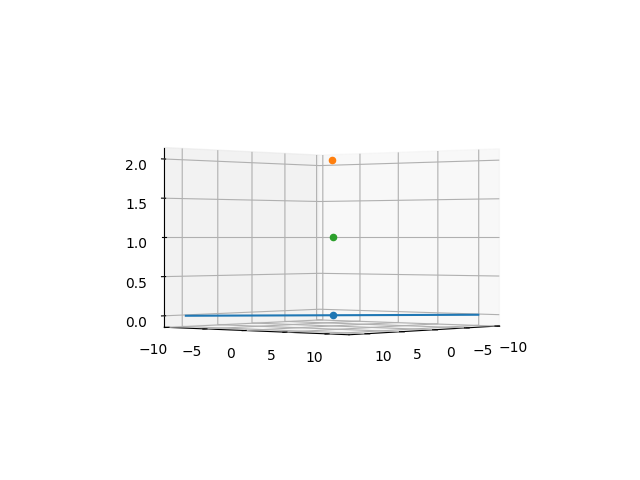
\includegraphics{fig2.png}

\problem{5}
We use the fact that the equation of a plane can be written

$$\bm{v} \cdot \bm{x} + d = 0$$

Solving for $d$,
$$
d = - \bm{v} \cdot {x}
$$

\lstinputlisting[language=Python, firstline=74, lastline=75]{lab1.py}

We find that $d=0$
Therefore,

$$
-x + y + 0 \cdot z = 0
$$

or

$$
x = y
$$



\end{document}


  